\ifthenelse{\equal{\lang}{ko}}{%
\begin{figure}[t]
  \centering
  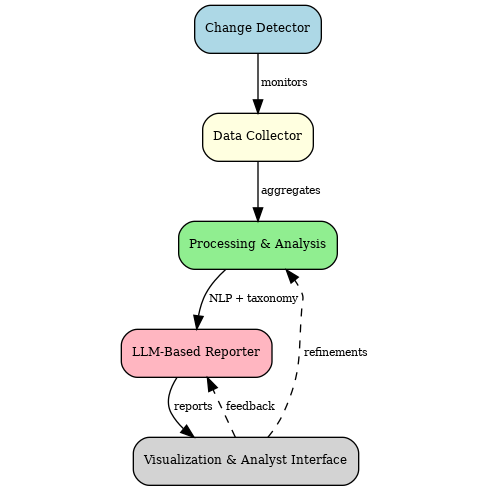
\includegraphics[width=0.9\linewidth]{fig-system_architecture.png}
  \caption{\textbf{LexSense 시스템 아키텍처.} 다섯 개의 모듈형 구성요소—탐지, 수집, 분석, 보고, 시각화—가 함께 작동하여 확장 가능하고, 다국어이며, 근거에 기반한 법률·정부 정보 접근을 가능하게 한다.}
  \label{fig:architecture}
\end{figure}

설계 목표는 세 가지이다: (1) \textbf{다국어 포용성(multilingual inclusiveness)} — 다양한 언어의 시민이 자신의 언어로 공공 정보에 접근할 수 있도록 함 \cite{conneau2020xlmr, xue2021mt5}; (2) \textbf{근거 기반 신뢰성(evidence-grounded reliability)} — 요약과 답변을 원문 근거에 연결하여 사실성을 보장함 \cite{lewis2020rag, maynez2020faithfulness}; (3) \textbf{투명성(transparency)} — 비전문가가 이해하고 검증할 수 있는 구조화된 설명 가능한 출력을 생성함 \cite{mitchell2021modelcards}.

\subsection{시스템 아키텍처}
그림~\ref{fig:architecture}은 시스템 아키텍처를 보여주며, 이는 다섯 개의 핵심 구성 요소로 이루어져 있다.
~\\
\textbf{1) 변화 탐지기(Change Detector):} 정부 포털, 법령·판례 데이터베이스, 공공 공지, 뉴스 매체를 지속적으로 모니터링하여 새로운 콘텐츠나 업데이트를 감지한다. 분산 크롤러와 스트리밍 파이프라인을 활용해 거의 실시간으로 후속 분석을 촉발한다 \cite{gama2014drift, niklaus2023multilegal}.
~\\
\textbf{2) 데이터 수집기(Data Collector):} 정책 데이터베이스, 법률 문서, 행정 공지 등 이질적 정보를 집계한다. API 기반 수집과 적응형 웹 스크래핑 모듈을 병행하여 다양한 관할권과 언어를 포괄한다 \cite{nllb2022}.
~\\
\textbf{3) 처리 및 분석 모듈(Processing and Analysis Module):} 개체 인식, 조항 추출, 이벤트 분류를 위해 다국어 NLP 파이프라인을 적용한다. Transformer 기반 다국어 인코더(mBERT, XLM-R)를 도메인 특화 분류체계와 결합하여 언어 간 전이를 통한 구조화된 표현을 가능케 한다 \cite{devlin2019bert, conneau2020xlmr}.
~\\
\textbf{4) LLM 기반 리포터(LLM-Based Reporter):} GPT-4, LLaMA-2 및 법률 도메인 특화 모델을 활용하여 구조화된 요약을 생성하고, 핵심 조항을 강조하며, 다중 출처 정보를 종합한다 \cite{openai2023gpt4, touvron2023llama2}. 또한 근거 구간에 기반한 검색 증강 생성(RAG)과 인간 피드백 루프를 적용하여 사실 정확성을 높이고 환각을 줄인다 \cite{lewis2020rag, ji2023hallucination}.
~\\
\textbf{5) 시각화 및 사용자 인터페이스(Visualization and User Interface):} 대시보드와 인터랙티브 요약을 제공하며, 평이한 언어(plain language) 설명과 근거 링크를 함께 표시한다. 비전문가의 이해와 신뢰를 돕도록 설계 원칙을 반영하였다 \cite{mitchell2021modelcards, ouyang2022instructgpt}.

\subsection{구현 세부사항}
시스템은 마이크로서비스 지향 아키텍처로 구현되어 모듈성과 확장성을 극대화한다. \textbf{데이터 수집:} 분산 크롤러가 Apache Kafka 큐에서 실행되어 50개 이상의 소스로부터 병렬적이고 내결함성 있는 데이터 수집을 수행한다 \cite{niklaus2023multilegal}. \textbf{전처리 파이프라인:} 다국어 인코더를 법률·정책 코퍼스에 파인튜닝하여 조항 추출 성능을 향상시키고 불필요한 잡음을 줄인다 \cite{devlin2019bert, conneau2020xlmr}. \textbf{의미 검색:} 문장 임베딩 기반 검색을 통해 다국어 근거 구간을 정렬한다 \cite{reimers2019sbert, reimers2020multilingual}. \textbf{피드백 루프:} 사용자 및 전문가 교정 내용은 기록 후 재학습에 반영되어 분류 정확도와 요약 품질을 점진적으로 향상시킨다. \textbf{재현성:} 전체 구현, 데이터 준비 스크립트, Docker 기반 환경을 GitHub에 공개하여 재현성을 보장한다 \cite{mitchell2021modelcards}.

\subsection{설계 원칙}
세 가지 설계 원칙이 아키텍처를 형성하였다: \textbf{(1) 모듈성(Modularity)} — 각 하위 시스템(탐지, 수집, 분석, 보고, 시각화)이 독립적으로 업데이트될 수 있어 새로운 LLM이나 다국어 데이터 소스와의 통합이 용이하다 \cite{devlin2019bert, conneau2020xlmr}; \textbf{(2) 효율성(Efficiency)} — 엔드투엔드 자동화를 통해 탐지와 요약 간의 지연을 최소화하여 준실시간 정보 접근을 가능케 한다 \cite{reimers2019sbert, lewis2020rag}; \textbf{(3) 투명성(Transparency)} — 산출물이 구조화되고 설명 가능하며 근거에 연결되도록 설계되어, 비전문가의 신뢰와 검증 가능성을 뒷받침한다 \cite{mitchell2021modelcards, maynez2020faithfulness}. 전체적으로, 본 설계는 확장성뿐 아니라 재현성, 사용성, 책임 있는 배포를 강조하며, 자동화된 정보 접근이 과학적으로 엄밀하면서도 다국어 공동체에 실질적으로 포용적일 수 있도록 한다 \cite{weidinger2021taxonomy, bommasani2021foundation}.

}{%


\begin{figure}[t]
  \centering
  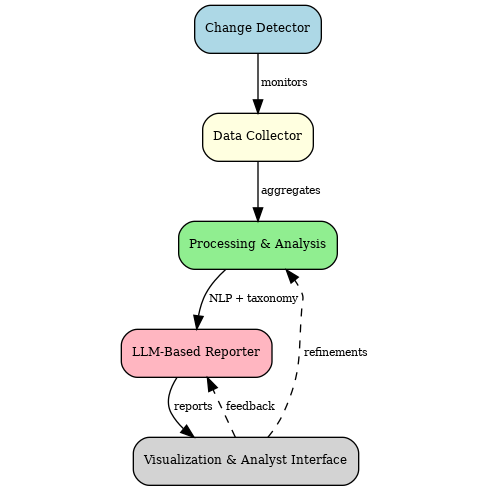
\includegraphics[width=0.9\linewidth]{fig-system_architecture}
  \caption{\textbf{LexSense System Architecture.} Five modular components—detection, collection, analysis, reporting, and visualization—work together to enable scalable, multilingual, and evidence-grounded access to legal and government information.}
  \label{fig:architecture}
\end{figure}


The design goals are threefold: (1) \textbf{multilingual inclusiveness}, so that citizens speaking diverse languages can access public information in their own language \cite{conneau2020xlmr, xue2021mt5}; (2) \textbf{evidence-grounded reliability}, linking summaries and answers to source evidence to ensure factuality \cite{lewis2020rag, maynez2020faithfulness}; and (3) \textbf{transparency}, generating structured, explainable outputs that non-experts can understand and verify \cite{mitchell2021modelcards}.


\subsection{System Architecture}
Figure~\ref{fig:architecture} illustrates the system's architecture, which is composed of five core components:
~\\
\textbf{1) Change Detector:} Continuously monitors government portals, statute and case-law databases, public notices, and news outlets for new or updated content. Using distributed crawlers and streaming pipelines, it triggers downstream analysis in near real time \cite{gama2014drift, niklaus2023multilegal}.
~\\
\textbf{2) Data Collector:} Aggregates heterogeneous information from policy databases, legal filings, and administrative notices. Both API-based ingestion and adaptive web-scraping modules are employed to ensure coverage across jurisdictions and languages \cite{nllb2022}.
~\\
\textbf{3) Processing and Analysis Module:} Applies multilingual NLP pipelines for entity recognition, clause extraction, and event classification. Transformer-based multilingual encoders (mBERT, XLM-R) are integrated with domain-specific taxonomies, enabling structured representation through cross-lingual transfer \cite{devlin2019bert, conneau2020xlmr}.
~\\
\textbf{4) LLM-Based Reporter:} Employs large language models (GPT-4, LLaMA-2, and legal-domain models) to generate structured summaries, highlight key clauses, and synthesize multi-source information \cite{openai2023gpt4, touvron2023llama2}. Retrieval-augmented generation (RAG) grounded in evidence spans, together with a human feedback loop, improves factual accuracy and reduces hallucinations \cite{lewis2020rag, ji2023hallucination}.
~\\
\textbf{5) Visualization and User Interface:} Provides dashboards and interactive summaries that present plain-language explanations alongside evidence links. Guided by design principles for trust and interpretability, the interface helps non-experts understand and trust the output \cite{mitchell2021modelcards, ouyang2022instructgpt}.

\subsection{Implementation Details}
The system is implemented using a microservice-oriented architecture to maximize modularity and scalability. \textbf{Data Ingestion:} distributed crawlers run on Apache Kafka queues, enabling parallel and fault-tolerant data collection from over 50 sources \cite{niklaus2023multilegal}. \textbf{Preprocessing Pipelines:} multilingual encoders are fine-tuned on legal and policy corpora to improve clause extraction and reduce noise \cite{devlin2019bert, conneau2020xlmr}. \textbf{Semantic Retrieval:} sentence-embedding-based retrieval aligns multilingual evidence spans \cite{reimers2019sbert, reimers2020multilingual}. \textbf{Feedback Loop:} user and expert corrections are logged and reintegrated into retraining, gradually refining classification accuracy and summary quality over time. \textbf{Reproducibility:} we release the full implementation, dataset preparation scripts, and Dockerized environments on GitHub \cite{mitchell2021modelcards}.



\subsection{Design Principles}
Three guiding principles shaped our architecture: \textbf{(1) Modularity}, where each subsystem—detection, collection, analysis, reporting, and visualization—can be independently updated, facilitating integration with emerging LLMs or multilingual data sources \cite{devlin2019bert, conneau2020xlmr}; \textbf{(2) Efficiency}, where end-to-end automation minimizes latency between detection and summarization, enabling near real-time information access \cite{reimers2019sbert, lewis2020rag}; and \textbf{(3) Transparency}, where outputs are structured, explainable, and evidence-linked, supporting trust and verifiability for non-experts \cite{mitchell2021modelcards, maynez2020faithfulness}. Overall, the design emphasizes not only scalability but also reproducibility, usability, and responsible deployment, ensuring that automated information access is both scientifically rigorous and practically inclusive for multilingual communities \cite{weidinger2021taxonomy, bommasani2021foundation}.


}
